\chapter{Design dei Benchmark e Risultati}
\label{sec:benchmark}

In questo capitolo verranno presentati i benchmark sviluppati per confrontare le performance delle soluzioni basate su CUDA e Vulkan. Verranno, inoltre, presentati i risultati ottenuti e le considerazioni che ne derivano.

\section{Benchmark}

Sono stati sviluppati due tipi di benchmark: uno per la somma di vettori e uno per la moltiplicazione di matrici sparse. Le misurazioni hanno tenuto conto sia del tempo di esecuzione su GPU che del tempo di trasferimento dei dati tra CPU e GPU. I calcoli sono stati eseguiti per tre tipi di dato: \verb|uint| (o \verb|u32|), \verb|float| (o \verb|f32|) e \verb|double| (o \verb|f64|). Questo ha permesso di capire come il codice ottimizzato in modo diverso da CUDA o Vulkan intacchi le performance in base al tipo di dato. 

La suite è stata eseguita sulla medesima macchina con la stessa versione dei driver, per garantire la coerenza dei risultati. In fig. \ref{fig:macchina} sono mostrate le caratteristiche della macchina: CPU Intel Xeon Platinum 8259CL e GPU NVIDIA Tesla T4 Tensor da 16 GB di memoria GDDR6.

\begin{figure}[ht]
    \centering
    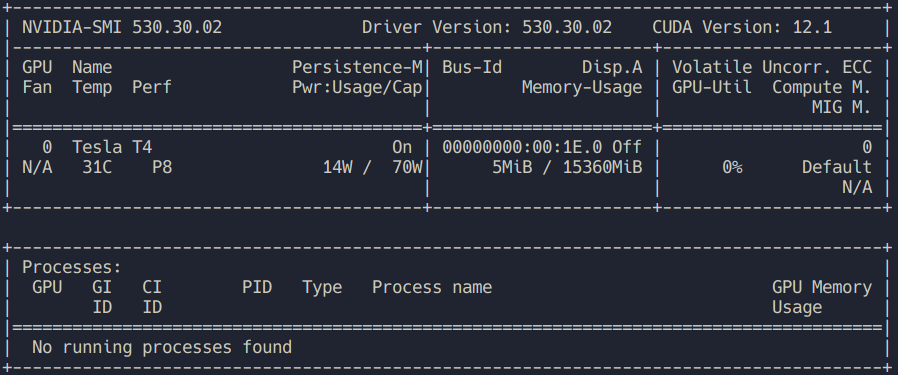
\includegraphics[width=.9\linewidth]{images/chapter4/macchina.png}
    \caption{Specifiche e driver della GPU su cui sono stati eseguiti i benchmark}
    \label{fig:macchina}
\end{figure}

Mentre all'inizio si era pensato di includere anche una versione dei benchmark su CPU, si è poi deciso di scartarli, in quanto non troppo rilevanti per il confronto tra le due soluzioni e poiché i tempi di esecuzione dell'intera suite erano già molto elevati. 

La compilazione di entrambi gli eseguibili è stata ottimizzata, tramite i flag dei rispettivi compilatori \ref{lis:comp_flags}, per ottenere il massimo delle performance. Sebbene questa accortezza non intacchi le prestazioni su GPU, è comunque necessaria per avere il throughput massimo della CPU per il trasferimento dei dati tra la memoria host e quella device.

\vspace{5mm}
\begin{lstlisting}[language=bash, caption=Impostazioni di compilazione CUDA e Rust, label=lis:comp_flags]
# Makefile CUDA
nvcc main.cu -o target/release/microbench_cuda -O3

# Cargo.toml
[profile.release]
strip = true
panic = "abort"
opt-level = 3
\end{lstlisting}
\vspace{5mm}

I tempi di esecuzione sono stati calcolati mediante funzioni fornite dalla libreria standard di entrambi i linguaggi, e sono stati ricalcolati più volte per ottenere una media più accurata. Per Vulkan si è usata la struct \verb|std::time::Instant| di Rust; mentre per CUDA si è sviluppato un timer che incorpora le funzioni \verb|cudaEventCreate| e \verb|cudaEventElapsedTime| \ref{lis:cuda_timer}, implementando API simili a quelle usate in Rust. I tempi risultati sono stati poi scritti su standard output specificando al tipo di benchmark di riferimento: come \verb|SUM VEC and COPY to host: 0.0000 ms| oppure \verb|MUL MAT and COPY to host: 0.0000 ms|. 
Inoltre ogni eseguibile accetta da linea di comando dei parametri per specificare la dimensione di vettori e matrici con cui eseguire i calcoli, il numero di iterazioni e il tipo di dato da testare.

\newpage
\vspace{5mm}
\begin{lstlisting}[language=C++, caption=Timer CUDA, label=lis:cuda_timer]
class Timer {
  cudaEvent_t start, stop;
  float elapsedTime = 0.0;

 public:
  void startTimer() {
    cudaEventCreate(&start);
    cudaEventRecord(start, 0);
  }

  void stopTimer() {
    cudaEventCreate(&stop);
    cudaEventRecord(stop, 0);
    cudaEventSynchronize(stop);
  }

  float calculateElapsed() {
    cudaEventElapsedTime(&elapsedTime, start, stop);
    return elapsedTime;
  }
};
\end{lstlisting}
\vspace{5mm}

Per automatizzare il processo di benchmarking, è stato scritto uno script in Python che richiama gli eseguibili dei benchmark e, leggendo tramite pipe lo standard output del programma, salva i risultati di ogni iterazione in un file json, infine calcola le medie dei tempi e riassume i risultati su un file CSV.



